\chapter{Webservice specifications}
\label{txt:webserviceSpec}

The Tellervo database is accessed solely through the webservice interface.  A webservice is an interface designed to be accessed by programs that send requests and receive responses.  Tellervo uses a style of HTTP+POX (Plain Old XML) to send and receive requests via a HTTP POST.  In simple terms the Tellervo client sends an XML document that describes the request via POST to the Tellervo server.  The server then reads the XML request, performs the request and then compiles the information that has been requested, finally returning the information to the client as another XML document.  The syntax of the XML document containing the request and response is determined by the Tellervo XML schema and makes heavy use of the TRiDaS XML schema for describing dendrochronological entities.

The Tellervo schema is the final authority on what is allowed in a request or response so if you find a conflict between this documentation and the schema then it is most likely because the documentation is out-of-date, or it's simply incorrect.  As you become familiar with the schema you'll probably find it easier to refer to it rather than this documentation to understand what is expecting.

This chapter outlines the basic syntax required for talking to the Tellero webservice and is largely aimed at developers who want to create new clients to interact with the Tellervo server.

\section{Basics of sending requests}
The webservice accepts requests via the POST mechanism of HTTP.  The simplest way to understand this is to think of this as a standard webpage.  If you add the following HTML code to a webpage it will give you a simple form.  If you type your XML request document into the form and click submit the Tellervo server will respond with an XML document containing the answer to your query.

\begin{lstlisting}
<form method="post" action="http://name.of.your.server/tellervo/">
  <textarea name="xmlrequest"/>
  <input type="submit" value="submit" >
</form>
\end{lstlisting}

A page with just such a form is available in the root of your Tellervo server installation as the page post.php.

When the response is viewed in a web browser, it will be rendered using a style sheet, but if you view the source code, you'll see the underlying XML document.  A simple HTML form like this can be handy for helping you send some rough requests to the server to help you understand how things work.

The Tellervo client (or any other client that wants to talk to the Tellervo server) does exactly this.  It sends XML formatted request documents to the server as POST requests, and the server returns an XML document containing the reply.  The client then reads the XML reply and displays the result to the user in any way it sees fit.


\section{Standard request/response}

The request XML document you send the server needs to validate against the Tellervo XML schema (available in the schema folder of your Tellervo server or in the /src/main/resources/schemas/ folder in the Subversion repository.  The schema is a detailed representation of what tags are allowed, when they are obligatory and what possible values they can contain.  We strongly suggest getting hold of an XML validation tool to help you check that the requests you send the server are valid.  The server will do the same and respond with an error message if it is not valid, but the textual error is a lot harder to understand than the graphic display of a desktop validation tool.

The general layout of the request file is as follows:

\begin{lstlisting}
<?xml version="1.0" encoding="UTF-8"?>
<tellervo xmlns="http://www.tellervo.org/schema/1.0" xmlns:gml="http://www.opengis.net/gml" xmlns:xlink="http://www.w3.org/1999/xlink" xmlns:tridas="http://www.tridas.org/1.2.2">
  <request type="">
    ...
    ...
  </request>
</tellervo>
\end{lstlisting}


\begin{itemize}
 \item \textbf{Line 1} contains the XML declaration and tells the server that we're using UTF-8 character encoding.  This is the only encoding currently supported.
 \item \textbf{Line 2} starts the root tag and defines the namespaces used by Tellervo.  The default namespace is the Tellervo schema itself, but it also refers to the TRiDaS, GML and XLink namespaces that Tellervo also makes use of.  Note that the default namespace may also be clarified with like the others as is used in a number of the examples that follow.  Only the namespaces that are used in the request are necessary though so if you're not referring to coordinate information for instance, you can safely leave out the GML namespace declaration.
 \item \textbf{Line 3} begins the request tag which contains the request itself. 
\end{itemize}






 

When you send such a request XML document to the Tellervo server the typical response returned is structured as follows:

\begin{lstlisting}
<?xml version="1.0" encoding="UTF-8"?>
<tellervo xmlns="http://www.tellervo.org/schema/1.0" xmlns:gml="http://www.opengis.net/gml" xmlns:xlink="http://www.w3.org/1999/xlink" xmlns:tridas="http://www.tridas.org/1.2.2">
  <header>
    ...
  </header>
  <content>
    ...
  </content>
</tellervo>
\end{lstlisting}

The header contains standard information about the request and also includes error and warning messages.  The content tag contains the actual data being returned.



\section{Authentication requests}

There are two methods for authenticating yourself against the Tellervo server: plain and secure.  We \emph{strongly} recommend you use the secure method as the user name and password are sent in plain text over the internet when using the plain method.  This goes against so much of the hard work we've put in to making the system secure.  It is quite likely that we will disable the plain authentication method by default in the future.  For now it will be left in place as it makes testing new clients much easier.  

For further details and discussion about the authentication design please see section \ref{txt:authentication}, page \pageref{txt:authentication}.

\subsection{Plain authentication}

If you \emph{still} want to go ahead and use plain authentication despite all the risks, then this is how you do it.

\begin{lstlisting}
<?xml version="1.0" encoding="UTF-8"?>
<tellervo xmlns="http://www.tellervo.org/schema/1.0" xmlns:tridas="http://www.tridas.org/1.3">
  <request type="plainlogin">
     <authenticate username="yourusername" password="yourpassword" />
  </request>
</tellervo>
\end{lstlisting}

\subsection{Secure authentication}

Although this is much more secure, it is also somewhat more complicated because it involves a challenge and response scheme using cryptographic nonces and hashes.  

The first step is for the client to request a nonce from the server.  This is done as follows:

\begin{lstlisting}
<?xml version="1.0" encoding="UTF-8"?>
<c:tellervo xmlns:c="http://www.tellervo.org/schema/1.0" xmlns:gml="http://www.opengis.net/gml" xmlns:xlink="http://www.w3.org/1999/xlink" xmlns:tridas="http://www.tridas.org/1.2.2">
  <c:request type="nonce" />
</c:tellervo>
\end{lstlisting}

The returned document will include a nonce header tag like this: \lstinline$<c:nonce seq="176378">97566d4d2e8b8c5696b6667fef8429f5</c:nonce>$.  Armed with your nonce you can then send a request to log in securely as follows:

\begin{lstlisting}
<?xml version="1.0" encoding="UTF-8"?>
<c:tellervo xmlns:c="http://www.tellervo.org/schema/1.0" xmlns:gml="http://www.opengis.net/gml" xmlns:xlink="http://www.w3.org/1999/xlink" xmlns:tridas="http://www.tridas.org/1.2.2">
  <c:request type="securelogin">
    <c:authenticate username="admin" cnonce="3f975c569f978731e570" snonce="97566d4d2e8b8c5696b6667fef8429f5" hash="d315ec50f7f1809492d5ef132ad4aa06" seq="176378" />
  </c:request>
</c:tellervo>
\end{lstlisting}

The authenticate attributes are filled as follows.  The username is simply the username for a user with permission to access the Tellervo server.  The cnonce (client nonce) is a random string of your choosing that is used in the hash.  The snonce (server nonce) is the nonce you've just obtained from the server.  The seq (sequence) is the value also obtained from the server.  Finally the hash is an MD5 hash of ``username:md5hashofpassword:snonce:cnonce''.  If all is well the server will respond with the details of the person that is logging in.

\subsection{Cookies and sessions}

The webservice uses a session cookie so that the user doesn't need to authenticate with each request.  The cookie lasts for up to 30 minutes of inactivity, after which point the server will request the user to re-authenticate before it will serve a request.  Any client attempting to access the Tellervo server will therefore need to handle cookies and be ready to respond to requests to re-authenticate.  

If a session does time out, a request to the server will result in an response with the header containing an error status with code `102' (see appendix \ref{txt:errorcodes}) and the nonce tag ready for the client to re-authenticate.  

\subsection{Logout}

The session cookie will ensure that a user is logged out after a period of inactivity, but if you want to force a logout you can simply use the following type of request:

\begin{lstlisting}
<?xml version="1.0" encoding="UTF-8"?>
<c:tellervo xmlns:c="http://www.tellervo.org/schema/1.0">
  <c:request type="logout">
</c:tellervo> 
\end{lstlisting}


\section{Reading records}

The method for reading records from the Tellervo database is largely the same for any of the types of data the server handles.  The basic template for a read request is as follows:

\begin{lstlisting}
<?xml version="1.0" encoding="UTF-8"?>
<c:tellervo xmlns:c="http://www.tellervo.org/schema/1.0">
  <c:request type="read" format=" ">
    <c:entity type=" " id=" " />
  </c:request>
</c:tellervo>
\end{lstlisting}

The entity type is one of: project; object; element; sample; radius; measurementSeries; derivedSeries; box; securityUser; or securityGroup.  The id attribute should be the database identifier for the entity you would like to read.  In Tellervo these are typically a UUID like this: 339d8ea6-7448-11e1-ad85-9b6d022add7a.  The format attribute should be one of: minimal; summary; standard; or comprehensive depending on how much detail you require about the entity.  Keep in mind that a comprehensive request is likely to take much longer to fulfill than a minimal request so it's best for your user, if you use the simplest request that fulfills your need.






\section{Deleting records}


\section{Creating records}






\subsection{Creating new series}

Due to the complications arising from the virtual measurement concept, creating new series in Tellervo is necessarily more complicated than any other of the TRiDaS entities.  The workflow required to create a new series is illustrated in figure \ref{fig:creatingNewMSeries}.

\begin{figure}[hbtp]
  \centering
  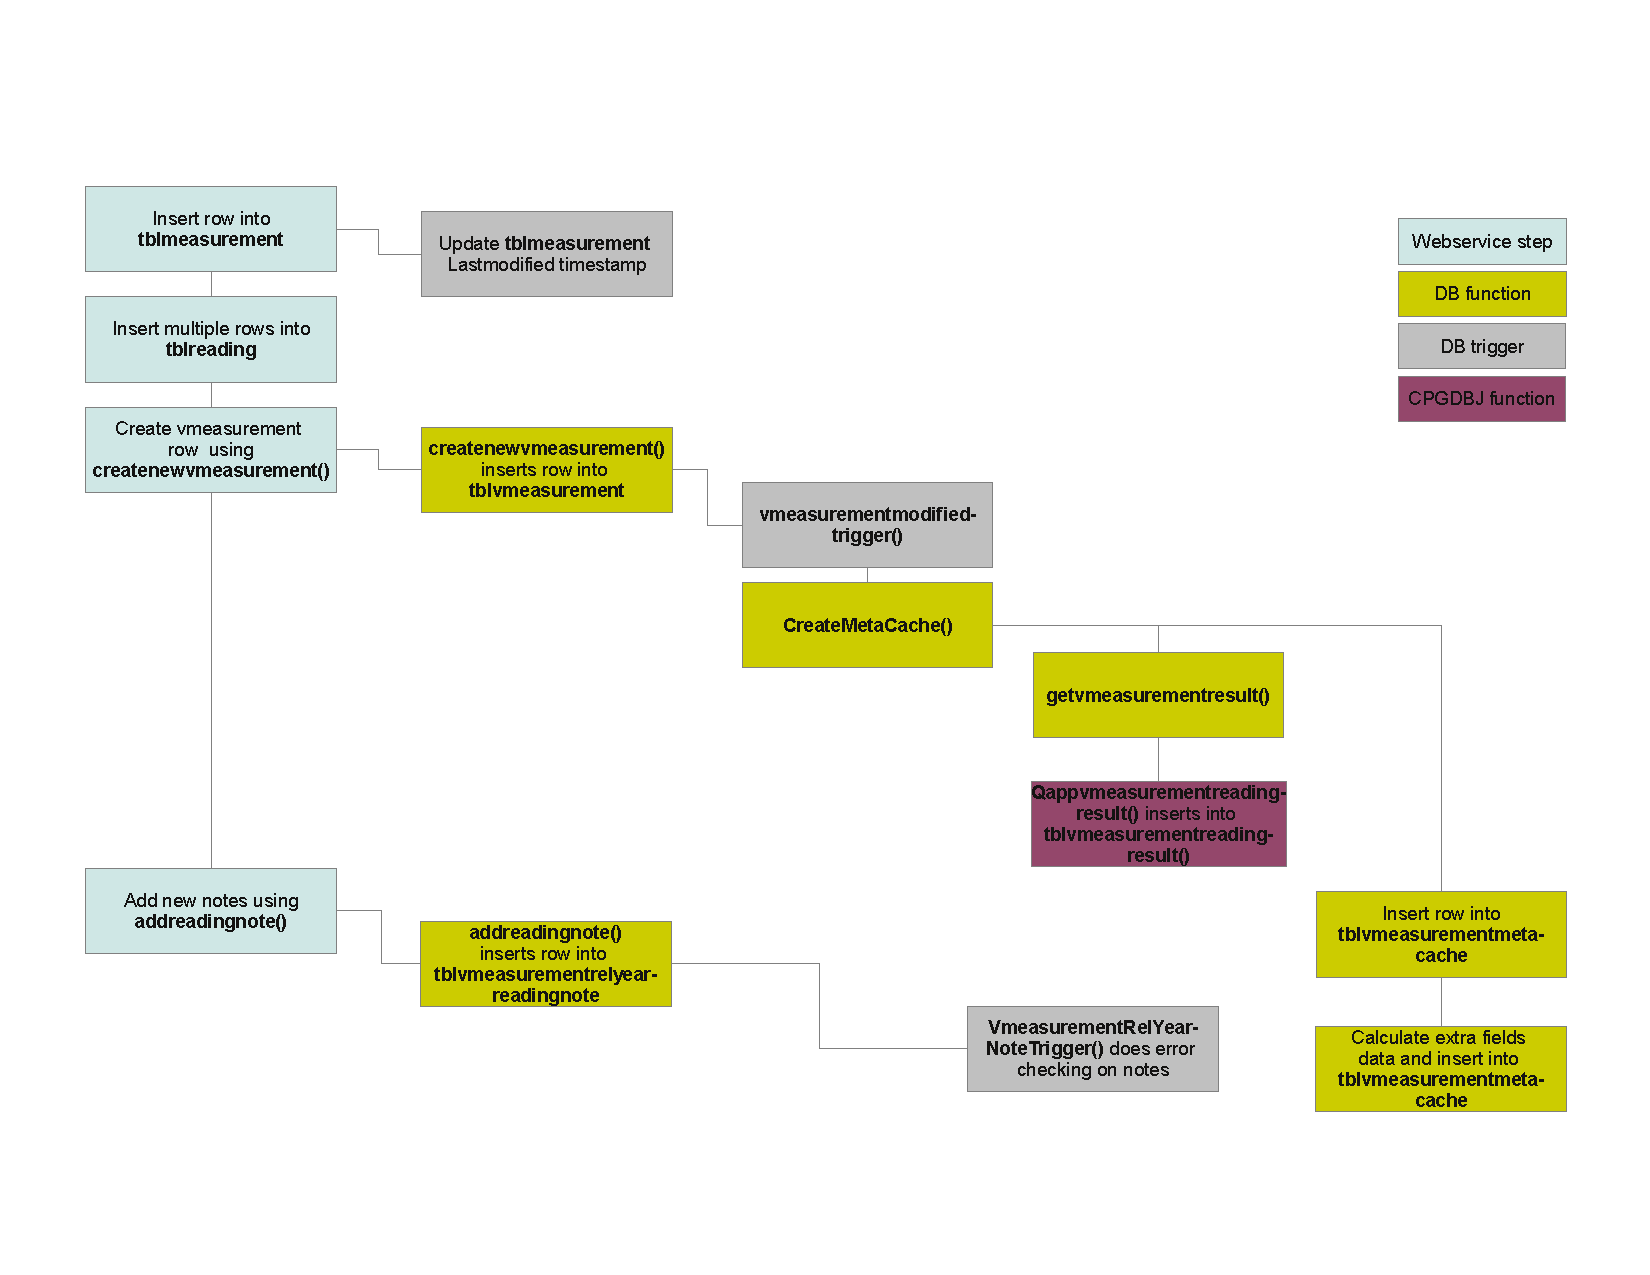
\includegraphics[width=0.8\textwidth]{Images/CreatingNewMSeriesWorkflow.pdf}
  \caption{Illustration of the steps that happen during the creation of a new measurement series. The stages are presented top to bottom in the approximate order in which they are executed.  The majority of the processing is done as a result of the database function createnewvmeasurement() being called by the webservice.}
  \label{fig:creatingNewMSeries}
\end{figure}

\begin{figure}[hbtp]
  \centering
  %\includegraphics[width=0.8\textwidth]{Images/EditingMSeriesWorkflow.pdf}
  \caption{Illustration of the steps that happen during the alteration of an existing measurement series. The stages are presented top to bottom in the approximate order in which they are executed.}
  \label{fig:editingNewMSeries}
\end{figure}

\begin{figure}[hbtp]
  \centering
  \includegraphics[width=0.8\textwidth]{Images/CreatingNewDSeriesWorkflow.pdf}
  \caption{Illustration of the steps that happen during the creation of a new derived series. The stages are presented top to bottom in the approximate order in which they are executed.  Depending on the type of derived series being created, a different database function is called to finish the new vmeasurement.}
  \label{fig:creatingNewMSeries}
\end{figure}

\begin{figure}[hbtp]
  \centering
  %\includegraphics[width=0.8\textwidth]{Images/EditingDSeriesWorkflow.pdf}
  \caption{Illustration of the steps that happen during the alteration of an existing derived series. The stages are presented top to bottom in the approximate order in which they are executed. Note that presently it is not possible to alter the parameters of a derived series.}
  \label{fig:editingNewMSeries}
\end{figure}



\section{Updating records}




\section{Reading and setting permissions}
\index{Developing!Permissions}
\index{Permissions}




\begin{lstlisting}
<request type="create">
  <permission>
      <permissionToCreate>true</permissionToCreate>  
      <permissionToRead>true</permissionToRead>
      <permissionToUpdate>true</permissionToUpdate>
      <permissionToDelete>true</permissionToDelete>
      <entity type="object" id="760a19e2-229c-11e1-8756-03b2aff2fe33"/>
      <securityGroup id="3"/>
  </permission>
</request>
\end{lstlisting}


\begin{lstlisting}
<request type="read">
  <permission>
      <entity type="object" id="760a19e2-229c-11e1-8756-03b2aff2fe33"/>
      <securityGroup id="3"/>
  </permission>
</request>
\end{lstlisting}


\begin{lstlisting}
<request type="update">
  <permission>
      <permissionToCreate>false</permissionToCreate>  
      <permissionToRead>false</permissionToRead>
      <permissionToUpdate>false</permissionToUpdate>
      <permissionToDelete>false</permissionToDelete>
      <entity type="object" id="136a70a6-566b-546b-a3ae-c48cb046e4cd"/>
      <securityUser id="1"/>
      <securityUser id="3"/>
  </permission>
</request>
\end{lstlisting}


\begin{lstlisting}
<request type="delete">
  <permission>
      <entity type="object" id="136a70a6-566b-546b-a3ae-c48cb046e4cd"/>
      <securityUser id="1"/>
  </permission>
</request>
\end{lstlisting}



